\section{Improved parallel composition of STGs}\label{sec_intro}


Parallel composition (synchronous product) of labelled
Petri nets is a fundamental operation in modular hardware design. It is
often used to combine models of subsystems into a model of the
whole system. In particular, there is a direct correspondence
between parallel composition of Signal Transition Graphs
(STGs), a class of labelled Petri nets used for modelling
asynchronous circuits, and connecting circuits by wires. Hence
performing this operation efficiently is important in practice.

Unfortunately, the standard definition of parallel composition almost always yields a `messy' Petri net, with many implicit places even when the component Petri nets did not have them. Some of these places are computationally cheap to remove (\eg duplicate places -- places with identical pre- and postsets). In general, however, for removing remaining implicit places one needs full-blown model checking, something infeasible if the resulting composition is large ~\cite{Schaefer06strategiesfor}.
Although implicit places do not have noticeable effect on tools based on state space exploration, such as \petrify~\cite{ckkly97}, the performance of tools that are based on structural methods, such as \desij~\cite{Sch07}, often deteriorates.

Consider the example in Fig.~\ref{fi-motivating-example1}. It
depicts an STG specifications of two components (a,b) and
the specification of the environment (c). The used short-hand
drawing notation for STGs is explained in
Sect.~\ref{sec_pn_basic}. The model of the behaviour of the
entire system can be obtained by constructing a parallel
composition of these three STGs, as shown in part (d) of
the figure. It contains a few implicit places
that are not duplicate places; intuitively, they appear due
to repeated causality specifications for every signal: the one
coming from the component where this signal is an output, and
others from the components where it is an input. Removing
these places yields a much `cleaner' STG, as
shown in Fig.~\ref{fi-motivating-example2}(d).

\begin{figure}[!tb]
    \centering
    \begin{minipage}[b]{0.4\columnwidth}
    \centering
        $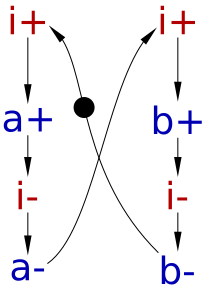
\includegraphics[scale=0.3]{EXPERIMENTS/stg/toggle}
        \atop
        \mbox{\rule[1.3em]{0em}{0em}(a) Toggle}$
        \\[0.5em]
        $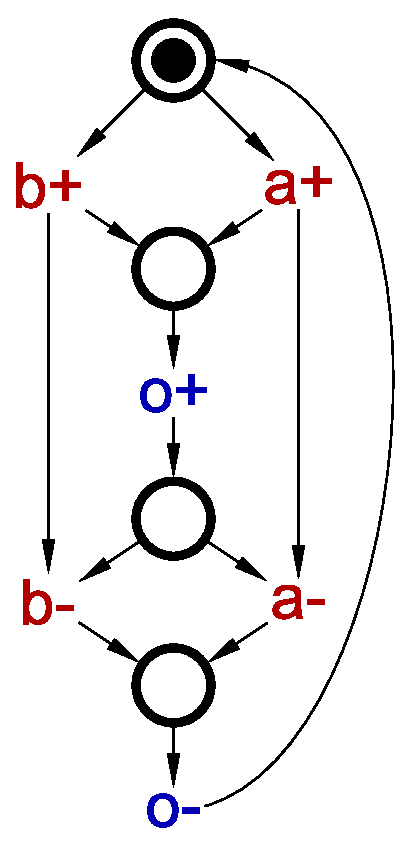
\includegraphics[scale=0.3]{EXPERIMENTS/stg/mix}
        \atop
        \mbox{\rule[1.3em]{0em}{0em}(b) Call}$
        \\[0.5em]
        $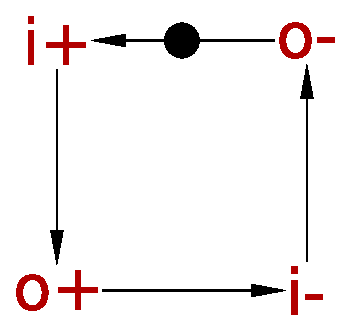
\includegraphics[scale=0.3]{EXPERIMENTS/stg/env}
        \atop
        \mbox{\rule[1.3em]{0em}{0em}(c) Environment}$
    \end{minipage}
    $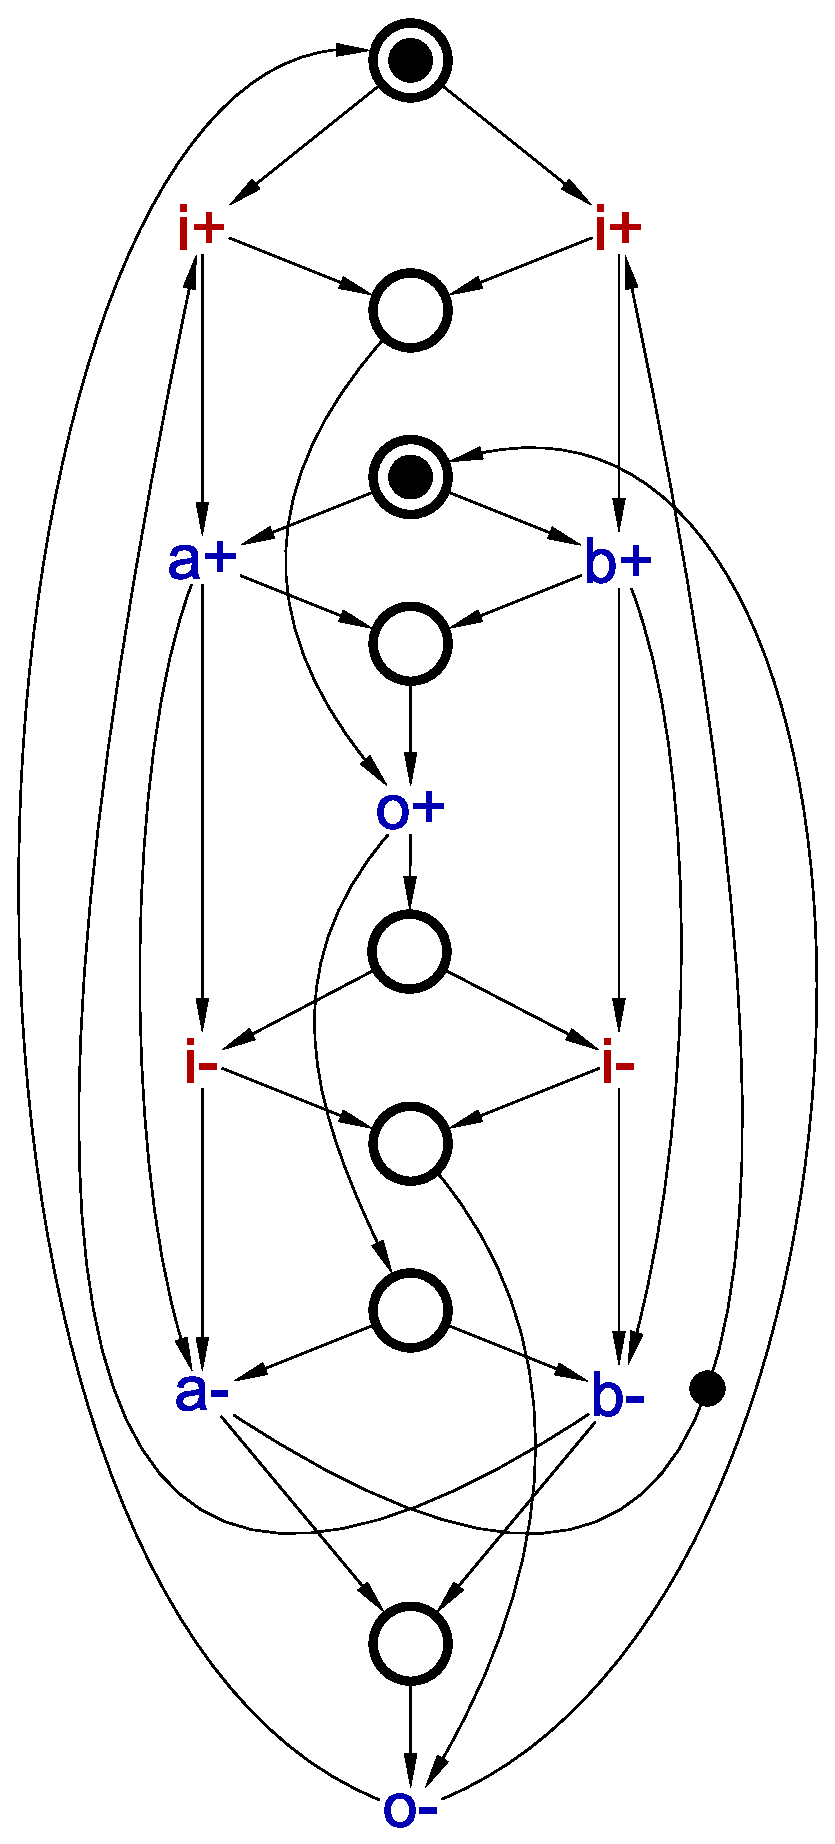
\includegraphics[scale=0.3]{EXPERIMENTS/stg/simple_standard}
    \atop
    \mbox{\rule[1.3em]{0em}{0em}(d) Composition}$
    \caption{\label{fi-motivating-example1}
        Example of standard STG composition.
    }
\end{figure}

\begin{figure}[!tb]
    \centering
    \begin{minipage}[b]{0.4\columnwidth}
        \centering
        $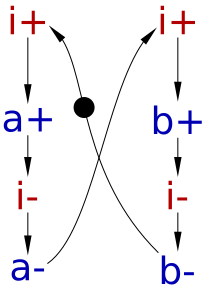
\includegraphics[scale=0.3]{EXPERIMENTS/stg/toggle_opt}
        \atop
        \mbox{\rule[1.3em]{0em}{0em}(a) Toggle}$
        \\[0.5em]
        $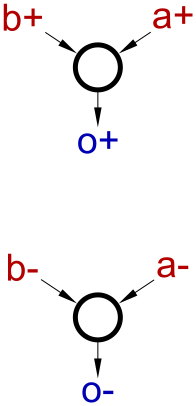
\includegraphics[scale=0.3]{EXPERIMENTS/stg/mix_opt}
        \atop
        \mbox{\rule[1.3em]{0em}{0em}(b) Call}$
        \\[0.5em]
        $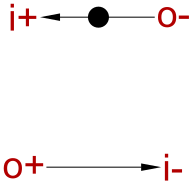
\includegraphics[scale=0.3]{EXPERIMENTS/stg/env_opt}
        \atop
        \mbox{\rule[1.3em]{0em}{0em}(c) Environment}$
    \end{minipage}
    $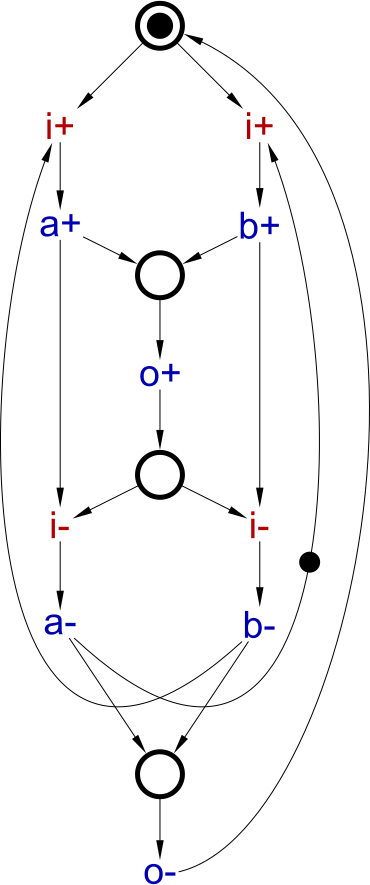
\includegraphics[scale=0.3]{EXPERIMENTS/stg/simple_improved}
    \atop
    \mbox{\rule[1.3em]{0em}{0em}(d) Composition}$
    \caption[Improved STG composition]{\label{fi-motivating-example2}
        Example of improved STG composition: the components are obtained from the corresponding ones in Fig.~\ref{fi-motivating-example1} by removing some places, and then the standard parallel composition is applied to these modified components.
    }
\end{figure}


One operation where implicit places matter is \emph{transition contraction}~\cite{vowo02lncs} -- a crucial part of the resynthesis approach. The idea is to hide the internal communication between the components by labelling the corresponding transitions as `dummy' (they correspond to signals $a$ and $b$ in our example), contract as many of these dummy transitions as possible, thus reducing the size of the STG, and resynthesise the obtained STG as a circuit. The result is often smaller than the original circuit due to removal of some signals. Transition contraction is normally performed on very large STGs, such as those corresponding to the whole control path of the circuit, and so, for efficiency, it has to be a structural operation. However, such structural contractions are not always possible (see Sect.~\ref{sec_pn_basic}), and implicit places in the pre-set and/or post-set of a transition can prevent contracting it, even if a contraction is possible after removing these implicit places. In the example in Fig.~\ref{fi-motivating-example1}(d), \desij~\cite{DesiJ} cannot contract any of the dummy transitions, even though it performs some structural tests for place redundancy. Yet, it is able to contract all the dummy transitions if the implicit places are removed, \ie when applied to the STG in Fig.~\ref{fi-motivating-example2}(d).

In Chapter \ref{chap:ParComp} we present a new method for computing the parallel composition of labelled Petri nets that generates fewer implicit places. It uses the \emph{freeness from computation interference (FCI)} assumption \cite{eber92} stating that it is impossible that when one component wants to produce an output it is prevented from doing so by another component not ready to receive it. Violation of the FCI assumption means that the behaviour of the composition does not correspond to that of an implied physical system. For example, an output of a circuit component cannot be physically disabled by another component that is not ready to receive this signal, and so producing this output will lead to a malfunction. However, the composition will be oblivious to the presence of the malfunction and behave as if such an output could not be produced.
Hence FCI is a basic correctness requirement -- whenever it is violated there is no point in computing a parallel composition since it would not characterise an intended behaviour. In practice, FCI is often guaranteed by construction, \eg its satisaction is guaranteed for the control path of a \balsa~\cite{EB-02} or \haste/\tangram~\cite{berkel91,haste-manual} specification of an asynchronous circuit. The idea of using the FCI condition is reminiscent of the method of input/output exposure in the synthesis by direct mapping described in~\cite{SBY-07} and of the correct by construction composition of Petri nets for circuit components and the environment used in the \ditopn tool~\cite{JF-00}.

The essence of the proposed method is illustrated by the example in Fig.~\ref{fi-motivating-example2}. Before computing a parallel composition, one can remove some of the places in the components (see (a--c) in Fig.~\ref{fi-motivating-example2}) and then compose the modified STGs. The precise conditions that allow us to remove a particular place will be stated in Sect.~\ref{se-main}. At this point we shall only mention that they are structural and thus can be efficiently checked. The method  guarantees that the number of places in the resulting Petri net is not larger and often much smaller (as the number of places in the composition is the total number of places in all the components), and, under the FCI assumption, the resulting behaviour is the same up to bisimularity. In the example, composing the modified components yields the STG in Fig.~\ref{fi-motivating-example2}(d), containing no implicit places. The modified components  may include unconstrained transitions and unbounded places and thus be non-implementable. Fortunately, this does not matter, as they are never used on their own, but only in composition with other components, and the resulting behaviour of the composition is guaranteed to correspond to that of the standard composition.

Resynthesis (Section \ref{sec:balsa-workflow}) of asynchronous circuits is the intended application of the proposed method. However, we envisage that it may find a much wider applicability since composition of labelled Petri nets is a fundamental operation and the FCI assumption often holds for practically important examples.
